\documentclass[tikz,border=5pt]{standalone}
\usetikzlibrary{hobby,spath3,intersections,arrows.meta,patterns}
\begin{document}
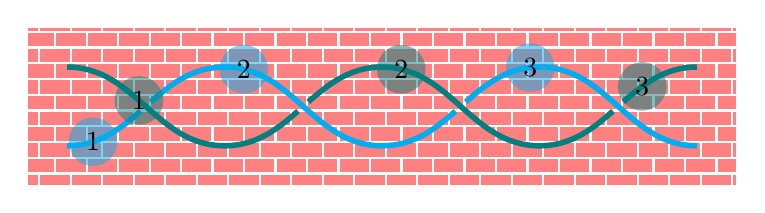
\begin{tikzpicture}[use Hobby shortcut]
    \draw[spath/save global=pathA] 
        (0,0) to[out=0,in=180] ++(2,1)
              to[out=0,in=180] ++(2,-1) 
              to[out=0,in=180] ++(2,1) 
              to[out=0,in=180] ++(2,-1);
    \draw[spath/save global=pathB] 
        (0,1) to[out=0,in=180] ++(2,-1)
              to[out=0,in=180] ++(2,1) 
              to[out=0,in=180] ++(2,-1) 
              to[out=0,in=180] ++(2,1);
    \tikzset{
        spath/.cd,
        split at intersections={pathA}{pathB},
        insert gaps after components={pathA}{5pt}{1,3}, %insert gaps
        join components={pathA}{3,5}, % remove the move operation
        get components of={pathA}\pathAcomponents, 
        insert gaps after components={pathB}{5pt}{2,4}, %insert gaps
        join components={pathB}{2,4}, % remove the move operation
        get components of={pathB}\pathBcomponents,
    }

    \fill[red!50!white] (-.5,-.5) rectangle (8.5,1.5); 
    \fill[pattern=bricks, pattern color=white] (-.5,-.5) rectangle (8.5,1.5);

    \foreach[count=\k] \cpt in \pathAcomponents { 
        \draw[cyan, line width=2pt,spath/use=\cpt]; 
        \node[fill=cyan, fill opacity=.5, circle, text opacity=1] at
        (spath cs:{\cpt} .3) {\(\k\)};
    }

    \foreach[count=\k] \cpt in \pathBcomponents { 
        \draw[teal, line width=2pt,spath/use=\cpt];
        \node[fill=teal, fill opacity=.5, circle, text opacity=1]
        at (spath cs:{\cpt} .3) {\(\k\)};
    }
\end{tikzpicture}
\end{document}